\section{Graph-Based Data Structures} 

  So far, arrays and hashing are the two most intuitive ways that we would store data. The next set of data structures not only store values, but it store the \textit{interactions} between these values. While it may not seem as natural to the new-comer, trees---and more generally, graphs---are a natural way to store real-world data. 

  At this point, you should be familiar with the concept of \textit{recursive algorithms}, which naturally appears in graphs (e.g. a subtree of a tree is a tree itself). Unlike the previous data structures, the elementary operations on graphs (e.g. insert, remove, etc.) are not as trivial, and so the conceptual difficulty significantly jumps from here.  

\subsection{Graphs}

  \begin{definition}[Undirected Graphs]
    An \textbf{undirected graph} $G(V, E)$ is a tuple, where $V = \{v_1, \ldots, v_n\}$ is the vertex set and $E = \{\{v_i, v_j\}\}$ is the edge set. 
    \begin{enumerate}
      \item The \textbf{degree} $d_v$ of a vertex $v$ is the number of edges incident to it. 
      \item A \textbf{path} is a sequence of vertices where adjacent vertices are connected by a path in $E$. It's \textbf{length} is the number of edges in the path. 
      \item A \textbf{cycle/circuit} is a path that has the same start and end. 
      \item A graph is \textbf{connected} if for every pair of vertices $e_i, e_j \in E$, there is a path from $e_i$ to $e_j$. 
      \item A \textbf{connected component} is a maximal subset of connected vertices. 
    \end{enumerate}
    The \textbf{size} of a graph is a tuple $(n, m) = (|V|, |E|)$. 
  \end{definition}

  \begin{definition}[Directed Graph]
    A \textbf{directed graph} $G(V, E)$ is a tuple, where $V = \{v_1, \ldots, v_n\}$ is the vertex set and $E = \{(v_i, v_j)\}$ is the edge set (note that it is a set of tuples, so $(i, j) \neq ( j, i)$).
    \begin{enumerate}
      \item The \textbf{in/out degree} $d_{v, i}, d_{v, o}$ of a vertex $v$ is the number of edges going in to or out from $v$. 
      \item A \textbf{path} is a sequence of vertices where adjacent vertices are connected by a path in $E$. It's \textbf{length} is the number of edges in the path. 
      \item A \textbf{cycle/circuit} is a path that has the same start and end. 
      \item A directed graph is \textbf{strongly connected} if for every pair of vertices $e_i, e_j \in E$, there is a path from $e_i$ to $e_j$.\footnote{Obviously, a connected undirected graph is also strongly connected.}
      \item A \textbf{strongly connected component} is a maximal subset of connected vertices. 
    \end{enumerate}
  \end{definition}

  In fact, from these definitions alone, we can solve an ancient puzzle called \textit{the Bridges of Konigsberg}. Euler, in trying to solve this problem, had invented graph theory. 

  \begin{example}[Bridges of Konigsberg]
    Is there a way to walk that crosses each bridge \textit{exactly} once? 

    \begin{figure}[H]
      \centering
      \begin{subfigure}[b]{0.48\textwidth}
      \centering
        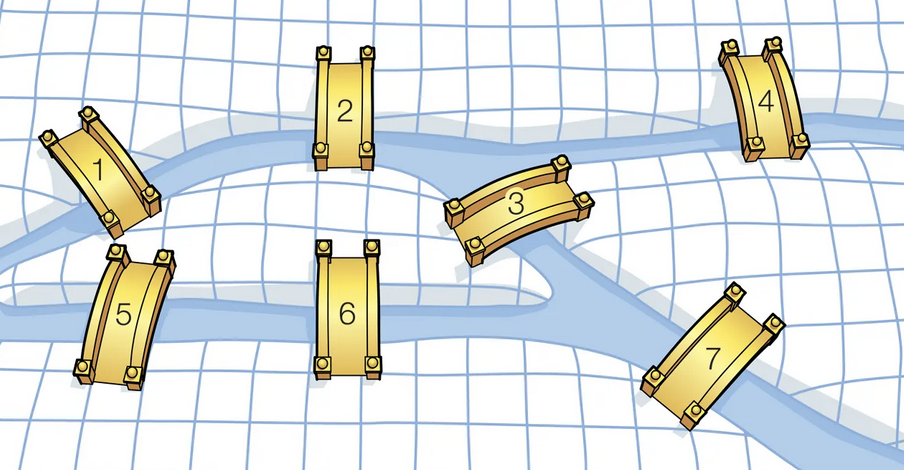
\includegraphics[scale=0.4]{img/bridges.png}
        \caption{Figure of the bridges of Konigsberg.}
        \label{fig:bridges}
      \end{subfigure}
      \hfill 
      \begin{subfigure}[b]{0.48\textwidth}
      \centering
        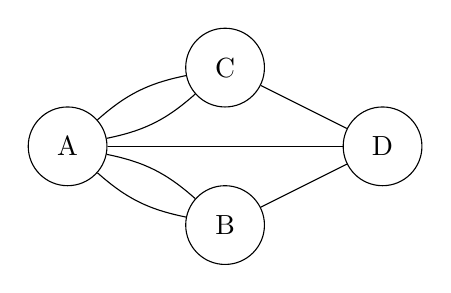
\begin{tikzpicture} 
          \tikzstyle{every node}=[circle, draw, minimum size=1cm]
          
          \node (A) at (0,0) {A};
          \node (B) at (2,-1) {B};
          \node (C) at (2,1) {C};
          \node (D) at (4,0) {D}; 
                
          \draw (A) to[bend left=15] (B);
          \draw (A) to[bend right=15] (B);
          \draw (A) to[bend left=15] (C);
          \draw (A) to[bend right=15] (C);
          \draw (A) -- (D);
          \draw (B) -- (D);
          \draw (C) -- (D);
        \end{tikzpicture}
        \caption{Graph representation. }
        \label{fig:graph_bridges}
      \end{subfigure}
      \caption{It can be decomposed into this undirected graph.}
      \label{fig:konigsberg}
    \end{figure}
     
    Euler's observation is that except for start and end points, a talk leaves any vertex by different edge that the incoming edge. Therefore, the degree (number of edges incident on it) must have an even number, so all but 2 vertices must have an even degree. Since every vertex has an odd degree, there is no way of doing it. 
  \end{example}

  In addition to the \textit{adjacency list} representation, another way in which we represent a directed graph is through \textit{adjacency matrices}. 

  \begin{definition}[Adjacency Matrix]
    In a finite directed graph $(V, E)$, we can construct a bijection from $V$ to the natural numbers and so we label each element in $V$ with $i \in \mathbb{N}$. Then, we can construct a matrix $A$ such that 
    \begin{equation}
      A_{ij} = \begin{cases} 1 & \text{ if } (i, j) \in E \\ 0 & \text{ if } (i, j) \not\in E \end{cases}
    \end{equation}
  \end{definition}

  \begin{example}[Adjacency List vs Matrix]
    Given a graph, we can completely represent it with a list of adjacent vertices for each vertex or an adjacency matrix. 
    \begin{center}
    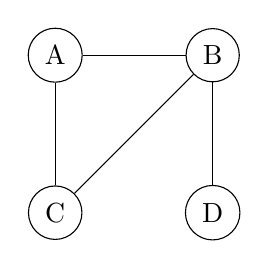
\begin{tikzpicture}
      \node[circle, draw] (C) at (0,0) {C};
      \node[circle, draw] (D) at (2,0) {D};
      \node[circle, draw] (B) at (2,2) {B};
      \node[circle, draw] (A) at (0,2) {A};

      \draw (A) -- (B);
      \draw (B) -- (C);
      \draw (A) -- (C);
      \draw (B) -- (D);
    \end{tikzpicture}
    \end{center}
    An adjacency list would look something like this 
    \[
    \begin{aligned}
    A &: B, C \\
    B &: A, C, D \\
    C &: A, B \\
    D &: B
    \end{aligned}
    \]
    and the adjacency matrix looks like this: 
    \begin{center}
    \begin{tikzpicture}
      \matrix[matrix of math nodes, nodes in empty cells,          column sep=-\pgflinewidth, row sep=-\pgflinewidth,          nodes={minimum size=7mm, anchor=center, outer sep=0pt}] (adjacency) {
        & |(a)| A & |(b)| B & |(c)| C & |(d)| D \\
        |(A)| A & 0 & 1 & 1 & 0 \\
        |(B)| B & 1 & 0 & 1 & 1 \\
        |(C)| C & 1 & 1 & 0 & 0 \\
        |(D)| D & 0 & 1 & 0 & 0 \\
      };
    \end{tikzpicture}
    \end{center}
  \end{example}

  While the adjacency matrix does have its advantages and has a cleaner form, usually in sparse graphs this is memory inefficient due to there being an overwhelming number of $0$s. 

  \begin{algo}[Insert Node/Edge in Graph]
    
  \end{algo}

  \begin{algo}[Remove Node/Edge in Graph]
    
  \end{algo}

  \begin{algo}[Contains in Graph]
    
  \end{algo} 

\subsection{Graph Traversal with DFS/BFS}

  Given two $v, s \in V$ either directed or undirected, how can we find a path from $v$ to $s$? We can do with either with DFS or BFS. 

  Now, in order to traverse this graph, we basically want to make an algorithm that starts at a node, prints it value, and then goes to all of its neighbors (which we can access through the adjacency list) to print them out. Thus, this is by nature recursive. We don't want the algorithm to loop around printing nodes infinitely often, so we must create a base case that tells the algorithm to not print out a node. It makes sense to create a set of visited nodes, which we can add to whenever we reach a new node. So, if we ever come onto a node that we have visited, we can just tell the function to do nothing. 

  \begin{algo}[Recursive Depth-First Search]
    The recursive implementation of Depth-First Search explores a graph by recursively visiting each unvisited neighbor, going as deep as possible along each branch before backtracking.
    \begin{algorithm}[H]
      \label{alg:dfs_recursive}
      \begin{algorithmic}[1]
        \Require{Graph $G(V, E)$, start vertex $s$}
        
        \Function{DFS-Recursive}{$G, s$}
          \State visited $\gets \emptyset$ \Comment{Initialize empty set of visited vertices}
          \State \Call{DFS-Visit}{$G, s$, visited}
        \EndFunction
        
        \Function{DFS-Visit}{$G, u$, visited}
          \State Add $u$ to visited
          \State \textit{/* Process vertex $u$ here */}
          \For{each neighbor $v$ of $u$ in $G$}
            \If{$v \notin$ visited}
              \State \Call{DFS-Visit}{$G, v$, visited}
            \EndIf
          \EndFor
        \EndFunction
      \end{algorithmic}
    \end{algorithm}
  \end{algo}

  Though recursion really makes this simple, we can construct an iterative approach that uses stacks. Note that in recursion, we are really making a call stack of different functions. We can be explicit about this by actually implementing a stack, which would store all the nodes that we have discovered, but not yet explored from )i.e. all the current nodes). At each iteration, we would pick a node to continue exploring, and since this is a DFS, we would want to implement a LIFO stack so that the last element we input in is the first thing that we should explore from, i.e. we always explore from the last node discovered. 

  \begin{algo}[Iterative Depth-First Search]
    The iterative implementation of Depth-First Search uses a stack to mimic the function call stack of the recursive implementation. It explores vertices in the same order as the recursive version.
    \begin{algorithm}[H]
      \label{alg:dfs_iterative}
      \begin{algorithmic}[1]
        \Require{Graph $G(V, E)$, start vertex $s$}
        
        \Function{DFS-Iterative}{$G, s$}
          \State visited $\gets \emptyset$ \Comment{Initialize empty set of visited vertices}
          \State stack $\gets$ empty stack
          \State Push $s$ onto stack
          \State Add $s$ to visited
          
          \While{stack is not empty}
            \State $u \gets$ Pop from stack
            \State \textit{/* Process vertex $u$ here */}
            
            \For{each neighbor $v$ of $u$ in $G$}
              \If{$v \notin$ visited}
                \State Add $v$ to visited
                \State Push $v$ onto stack
              \EndIf
            \EndFor
          \EndWhile
        \EndFunction
      \end{algorithmic}
    \end{algorithm}
  \end{algo}

  \begin{example}[DFS Walkthrough]
    Let's conduct DFS on the following graph. 

    \begin{figure}[H]
      \centering
      \begin{subfigure}[b]{0.48\textwidth}
        \centering
        \begin{tikzpicture}[
            node/.style={circle, draw, minimum size=0.8cm},
            arrow/.style={-Stealth, thick}
          ]
          % Define the nodes
          \node[node, red] (A) at (0,0) {A};
          \node[node] (B) at (3,0) {B};
          \node[node] (C) at (3,-2) {C};
          \node[node] (D) at (0,-2) {D};

          % Connect the nodes with directed edges
          \draw[arrow, red] (A) -- (B);
          \draw[arrow] (B) -- (C);
          \draw[arrow] (C) -- (D);
          \draw[arrow] (D) -- (A);
          \draw[arrow] (A) -- (C);
          \draw[arrow] (B) -- (D);
        \end{tikzpicture}
        \caption{You start at $A$ and you add it to your visited set $V = \{A\}$. You look at your neighbors and find that you can explore $B$ or $C$. Let's randomly choose to explore $B$ but keep in mind that you haven't finished exploring from $B$ since there's $C$ left. }
      \end{subfigure}
      \hfill 
      \begin{subfigure}[b]{0.48\textwidth}
        \centering
        \begin{tikzpicture}[
            node/.style={circle, draw, minimum size=0.8cm},
            arrow/.style={-Stealth, thick}
          ]
          % Define the nodes
          \node[node, red] (A) at (0,0) {A};
          \node[node, red] (B) at (3,0) {B};
          \node[node] (C) at (3,-2) {C};
          \node[node] (D) at (0,-2) {D};

          % Connect the nodes with directed edges
          \draw[arrow, red] (A) -- (B);
          \draw[arrow] (B) -- (C);
          \draw[arrow] (C) -- (D);
          \draw[arrow] (D) -- (A);
          \draw[arrow] (A) -- (C);
          \draw[arrow, red] (B) -- (D);
        \end{tikzpicture}
        \caption{You add $B$ to visited $V = \{A, B\}$ and look at your neighbors $C$ and $D$. Let's just choose $D$ randomly but keep in mind that you have $C$ to explore later, so you haven't finished exploring from $B$ either. Therefore both $A$ and $B$ are both still on your exploration stack.}
      \end{subfigure}

      \begin{subfigure}[b]{0.48\textwidth}
        \centering
        \begin{tikzpicture}[
            node/.style={circle, draw, minimum size=0.8cm},
            arrow/.style={-Stealth, thick}
          ]
          % Define the nodes
          \node[node, red] (A) at (0,0) {A};
          \node[node, red] (B) at (3,0) {B};
          \node[node] (C) at (3,-2) {C};
          \node[node, red] (D) at (0,-2) {D};

          % Connect the nodes with directed edges
          \draw[arrow, red] (A) -- (B);
          \draw[arrow] (B) -- (C);
          \draw[arrow] (C) -- (D);
          \draw[arrow, red] (D) -- (A);
          \draw[arrow] (A) -- (C);
          \draw[arrow, red] (B) -- (D);
        \end{tikzpicture}
        \caption{You add $D$ to visited $V = \{A, B, D\}$. You look at your neighbors and see that you can explore $A$. However it is already in your visited set. Since there are no more neighbors to explore to, you are done exploring from $D$ and don't need to look at it anymore. }
      \end{subfigure}
      \hfill 
      \begin{subfigure}[b]{0.48\textwidth}
        \centering
        \begin{tikzpicture}[
            node/.style={circle, draw, minimum size=0.8cm},
            arrow/.style={-Stealth, thick}
          ]
          % Define the nodes
          \node[node, red] (A) at (0,0) {A};
          \node[node, red] (B) at (3,0) {B};
          \node[node] (C) at (3,-2) {C};
          \node[node, red] (D) at (0,-2) {D};

          % Connect the nodes with directed edges
          \draw[arrow, red] (A) -- (B);
          \draw[arrow, red] (B) -- (C);
          \draw[arrow] (C) -- (D);
          \draw[arrow, red] (D) -- (A);
          \draw[arrow] (A) -- (C);
          \draw[arrow, red] (B) -- (D);
        \end{tikzpicture}
        \caption{Therefore you look back to where you came from: $B$, and continue exploring from $B$. You go back to $B$ and look at the other nodes you must explore. You've already done $D$ and the only remaining is $C$, which isn't in your visited. }
      \end{subfigure}

      \begin{subfigure}[b]{0.48\textwidth}
        \centering
        \begin{tikzpicture}[
            node/.style={circle, draw, minimum size=0.8cm},
            arrow/.style={-Stealth, thick}
          ]
          % Define the nodes
          \node[node, red] (A) at (0,0) {A};
          \node[node, red] (B) at (3,0) {B};
          \node[node, red] (C) at (3,-2) {C};
          \node[node, red] (D) at (0,-2) {D};

          % Connect the nodes with directed edges
          \draw[arrow, red] (A) -- (B);
          \draw[arrow, red] (B) -- (C);
          \draw[arrow, red] (C) -- (D);
          \draw[arrow, red] (D) -- (A);
          \draw[arrow] (A) -- (C);
          \draw[arrow, red] (B) -- (D);
        \end{tikzpicture}
        \caption{Add $C$ to visited $V = \{A, B, C, D\}$. You look at your neighbors and see $D$ as the only neighbor to explore. However, you have already explored $D$ and so there are no more neighbors left. Therefore you go back to the node you came from: $B$.}
      \end{subfigure}
      \hfill 
      \begin{subfigure}[b]{0.48\textwidth}
        \centering
        \begin{tikzpicture}[
            node/.style={circle, draw, minimum size=0.8cm},
            arrow/.style={-Stealth, thick}
          ]
          % Define the nodes
          \node[node, red] (A) at (0,0) {A};
          \node[node, red] (B) at (3,0) {B};
          \node[node, red] (C) at (3,-2) {C};
          \node[node, red] (D) at (0,-2) {D};

          % Connect the nodes with directed edges
          \draw[arrow, red] (A) -- (B);
          \draw[arrow, red] (B) -- (C);
          \draw[arrow, red] (C) -- (D);
          \draw[arrow, red] (D) -- (A);
          \draw[arrow, red] (A) -- (C);
          \draw[arrow, red] (B) -- (D);
        \end{tikzpicture}
        \caption{You continue exploring from $B$. There are no more nodes to explore, so you go back to the node you came from $A$. You see that the only remaining neighbor to explore is $C$, but it is already in visited, so you don't need to explore it. You are done.}
      \end{subfigure}

      \caption{Walkthrough of DFS on a small graph. The iterative and recursive approaches are identical.}
      \label{fig:dfs_example}
    \end{figure}
  \end{example}

  \begin{theorem}[Runtime of DFS]
    The runtime of DFS is $O(n+m)$. 
  \end{theorem}
  \begin{proof}
    The runtime complexity of this search is $O(N + M)$ because first, the while loop loops at most over the $N$ nodes. The for loop may loop over $M$ edges, but this is a bit pessemistic in bound. Rather, we can view it as looping over neighbors of each node at most exactly once, and so it considers every edge twice, meaning that the for loop will get called $2M$ times in the entire algorithm. So $N + 2M = O(N + M)$. 
  \end{proof}

  \begin{example}[DFS in a Maze]
    We can represent a grid graph, like a maze, with a two dimensional array that stores whether it is connected north, east, south, and west, where boolean of true represents that there is a wall, and false means there isn't a wall (so connected). 

    \begin{figure}[H]
      \centering
      \begin{subfigure}[b]{0.48\textwidth}
      \centering
        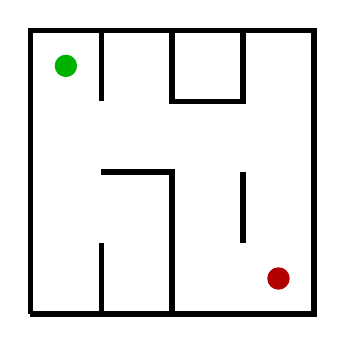
\begin{tikzpicture}[scale=0.9]
          % Outer boundary
          \draw[line width=2pt] (0,0) -- (4,0) -- (4,4) -- (0,4) -- (0,0);
          
          % Internal walls
          % Top section
          \draw[line width=2pt] (1,4) -- (1,3);
          \draw[line width=2pt] (2,4) -- (2,3) -- (3,3) -- (3,4);
          
          % Middle section
          \draw[line width=2pt] (1,2) -- (2,2) -- (2,1);
          \draw[line width=2pt] (3,2) -- (3,1);
          
          % Bottom section
          \draw[line width=2pt] (1,1) -- (1,0);
          \draw[line width=2pt] (2,1) -- (2,0);
          
          % Entry and exit points (just colored circles)
          \filldraw[green!70!black] (0.5,3.5) circle (0.15);
          \filldraw[red!70!black] (3.5,0.5) circle (0.15);
        \end{tikzpicture}
        \caption{4×4 maze representation}
        \label{fig:maze}
      \end{subfigure}
      \hfill 
      \begin{subfigure}[b]{0.48\textwidth}
      \centering
        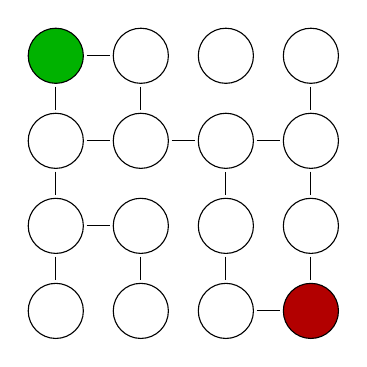
\begin{tikzpicture}[
          scale=0.9,
          node/.style={circle, draw, minimum size=0.7cm},
          edge/.style={draw, -, shorten >=1pt, shorten <=1pt}
        ]
          % Create a 4x4 graph for the new maze
          % Top row
          \node[node, fill=green!70!black, text=white] (A) at (0,3.6) {};
          \node[node] (B) at (1.2,3.6) {};
          \node[node] (C) at (2.4,3.6) {};
          \node[node] (D) at (3.6,3.6) {};
          
          % Second row
          \node[node] (E) at (0,2.4) {};
          \node[node] (F) at (1.2,2.4) {};
          \node[node] (G) at (2.4,2.4) {};
          \node[node] (H) at (3.6,2.4) {};
          
          % Third row
          \node[node] (I) at (0,1.2) {};
          \node[node] (J) at (1.2,1.2) {};
          \node[node] (K) at (2.4,1.2) {};
          \node[node] (L) at (3.6,1.2) {};
          
          % Bottom row
          \node[node] (M) at (0,0) {};
          \node[node] (N) at (1.2,0) {};
          \node[node] (O) at (2.4,0) {};
          \node[node, fill=red!70!black, text=white] (P) at (3.6,0) {};
          
          % Add edges based on available paths in the maze
          % Vertical connections
          \draw[edge] (A) -- (E);
          \draw[edge] (E) -- (I);
          \draw[edge] (I) -- (M);
          \draw[edge] (G) -- (H);
          
          \draw[edge] (B) -- (F);
          
          \draw[edge] (D) -- (H);
          \draw[edge] (H) -- (L);
          \draw[edge] (L) -- (P);
          
          \draw[edge] (J) -- (N);
          
          % Horizontal connections
          \draw[edge] (A) -- (B);
          
          \draw[edge] (E) -- (F);
          \draw[edge] (F) -- (G);
          \draw[edge] (K) -- (G);
          \draw[edge] (K) -- (O);
          
          \draw[edge] (I) -- (J);
          
          \draw[edge] (O) -- (P);
        \end{tikzpicture}
        \caption{Graph representation of the maze.}
        \label{fig:maze-graph}
      \end{subfigure}
      \caption{A 4×4 maze (left) and its corresponding graph representation (right). Start and end points are shown in green and red respectively.}
      \label{fig:maze-and-graph}
    \end{figure}

    But remember that in a tree traversal, we recursively searched down and down until we hit a null node, in which case we backtrack up to look in another branch. For graphs, this is a bit more complicated, since we could go in loops. Therefore, we want to keep track of all the visited nodes to avoid infinite recursion. We have three base cases: 
    \begin{enumerate}
      \item If we search off the grid, then this is not a valid path 
      \item If we already explored here, then we don't want to repeat it 
      \item If we reached the goal of the maze, then we output the length of the path. 
    \end{enumerate}
    The recursive case would take each node and recurse on its 4 adjacent neighbors, if they are connected. Note that this algorithm recurses on each of the $N$ nodes $4$ times (for each direction, and each recursive call is $O(1)$), so the complexity is $O(N)$. 
  \end{example}

  Note that the main idea of DFS is to always explore a new adjacent vertex if possible, and if not, then backtrack to the most recent vertex adjacent to an unvisited vertex and continue. On the contrary, the main idea of BFS is to explore \textit{all} your neighbors before you visit any of your neighbors' neighbors. It exhaustively searches for the closest regions of your search space before you look any further. Unlike DFS, which finds the some arbitrary path to a node, BFS finds the shortest (perhaps non-unique) path to a node. This can be simply done with a queue. 

  \begin{algo}[Iterative Breadth-First Search]
    Breadth-First Search (BFS) explores a graph by visiting all neighbors at the current depth before moving to nodes at the next depth level. It uses a queue to process nodes in the order they are discovered.
    \begin{algorithm}[H]
      \label{alg:bfs}
      \begin{algorithmic}[1]
        \Require{Graph $G(V, E)$, start vertex $s$}
        
        \Function{BFS}{$G, s$}
          \State visited $\gets \emptyset$ \Comment{Initialize empty set of visited vertices}
          \State queue $\gets$ empty queue
          \State Enqueue $s$ onto queue
          \State Add $s$ to visited
          
          \While{queue is not empty}
            \State $u \gets$ Dequeue from queue \Comment{Get the next vertex to process}
            \State \textit{/* Process vertex $u$ here */}
            
            \For{each neighbor $v$ of $u$ in $G$}
              \If{$v \notin$ visited}
                \State Add $v$ to visited
                \State Enqueue $v$ onto queue
              \EndIf
            \EndFor
          \EndWhile
        \EndFunction
      \end{algorithmic}
    \end{algorithm}
  \end{algo}

  \begin{example}[BFS Walkthrough]
    Let's conduct BFS on the following graph. 

    \begin{figure}[H]
      \centering
      \begin{subfigure}[b]{0.48\textwidth}
        \centering
        \begin{tikzpicture}[
            node/.style={circle, draw, minimum size=0.8cm},
            arrow/.style={-Stealth, thick}
          ]
          % Define the nodes
          \node[node, red] (A) at (0,0) {A};
          \node[node, blue] (B) at (3,0) {B};
          \node[node, blue] (C) at (3,-2) {C};
          \node[node] (D) at (0,-2) {D};
          % Connect the nodes with directed edges
          \draw[arrow, blue] (A) -- (B);
          \draw[arrow] (B) -- (C);
          \draw[arrow] (C) -- (D);
          \draw[arrow] (D) -- (A);
          \draw[arrow, blue] (A) -- (C);
          \draw[arrow] (B) -- (D);
        \end{tikzpicture}
        \caption{You start at $A$ and you add it to your visited set $V = \{A\}$ and to your queue $[A]$. You immediately dequeue $A$ from the queue and look at all neighbors of $A$, which are $B$ and $C$. You add both to your queue in some random order, say $B$ first. }
      \end{subfigure}
      \hfill 
      \begin{subfigure}[b]{0.48\textwidth}
        \centering
        \begin{tikzpicture}[
            node/.style={circle, draw, minimum size=0.8cm},
            arrow/.style={-Stealth, thick}
          ]
          % Define the nodes
          \node[node, red] (A) at (0,0) {A};
          \node[node, red] (B) at (3,0) {B};
          \node[node, blue] (C) at (3,-2) {C};
          \node[node, blue] (D) at (0,-2) {D};
          % Connect the nodes with directed edges
          \draw[arrow, red] (A) -- (B);
          \draw[arrow, red] (B) -- (C);
          \draw[arrow, blue] (C) -- (D);
          \draw[arrow] (D) -- (A);
          \draw[arrow, blue] (A) -- (C);
          \draw[arrow, blue] (B) -- (D);
        \end{tikzpicture}
        \caption{You deque $B$ and see that the adjacent nodes are $C$ and $D$. $C$ is already in your queue (check with visited set, which is $O(1)$), so you do not put it into your queue and can mark the corresponding edges as explored. You do put $D$ into the queue.}
      \end{subfigure}
      \begin{subfigure}[b]{0.48\textwidth}
        \centering
        \begin{tikzpicture}[
            node/.style={circle, draw, minimum size=0.8cm},
            arrow/.style={-Stealth, thick}
          ]
          % Define the nodes
          \node[node, red] (A) at (0,0) {A};
          \node[node, red] (B) at (3,0) {B};
          \node[node, red] (C) at (3,-2) {C};
          \node[node, blue] (D) at (0,-2) {D};
          % Connect the nodes with directed edges
          \draw[arrow, red] (A) -- (B);
          \draw[arrow, red] (B) -- (C);
          \draw[arrow, red] (C) -- (D);
          \draw[arrow, blue] (D) -- (A);
          \draw[arrow, red] (A) -- (C);
          \draw[arrow, blue] (B) -- (D);
        \end{tikzpicture}
        \caption{Next you dequeue $C$ since this is first seen from $A$. You explore from here and look at the neighbors, which is $D$. However, $D$ is already in your queue from $B$, so you skip it. There are no more neighbors to explore from $C$, so we look at the queue again.}
      \end{subfigure}
      \hfill 
      \begin{subfigure}[b]{0.48\textwidth}
        \centering
        \begin{tikzpicture}[
            node/.style={circle, draw, minimum size=0.8cm},
            arrow/.style={-Stealth, thick}
          ]
          % Define the nodes
          \node[node, red] (A) at (0,0) {A};
          \node[node, red] (B) at (3,0) {B};
          \node[node, red] (C) at (3,-2) {C};
          \node[node, red] (D) at (0,-2) {D};
          % Connect the nodes with directed edges
          \draw[arrow, red] (A) -- (B);
          \draw[arrow, red] (B) -- (C);
          \draw[arrow, red] (C) -- (D);
          \draw[arrow, red] (D) -- (A);
          \draw[arrow, red] (A) -- (C);
          \draw[arrow, red] (B) -- (D);
        \end{tikzpicture}
        \caption{You dequeue $D$ and look at the neighbors. The only neighbor is $A$ and it is already in visited, so we can skip this and mark the corresponding edge as explored. Since there are no more nodes to explore in our queue, this concludes BFS.}
      \end{subfigure}
      \caption{Walkthrough of BFS on a small graph. Blue represents the nodes/edges that are in our queue and red represents the nodes/edges that we have finished exploring.}
      \label{fig:bfs_example}
    \end{figure}
  \end{example}


  \begin{theorem}[Runtime of BFS]
    The runtime of BFS is $O(n+m)$. 
  \end{theorem}
  \begin{proof}
    To get the running time, we know that each vertex is popped only once from the queue, giving us $O(n)$. For each pop, we are exploring all the neighbors of $V$. 
    \begin{align}
      O \bigg( \sum_{v \in V} | \text{neighbors of } v| + 1\bigg) & = O \bigg( \sum_{v \in V} d_v + 1 \bigg) \\
                                           & = O (2 |E| + |V|) = O(m + n )
    \end{align}
    which is linear in input size!  
  \end{proof}

  The more straightforward application is in reachability. 

  \begin{example}[Reachability]
    Given a directed graph and a node $v$, find all nodes that are reachable from $v$. 
  \end{example}

  \begin{definition}[Search Trees]
    Once we have traversed a graph using BFS or DFS, we can label the directed path that this traversal algorithm takes into a \textbf{search tree}. 

    \begin{figure}[H]
      \centering
      \begin{subfigure}[b]{0.48\textwidth}
      \centering
        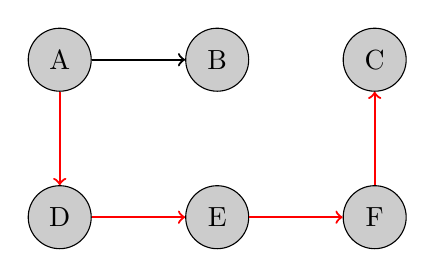
\begin{tikzpicture}[
            node/.style={circle, draw, fill=gray!40, minimum size=0.8cm},
            edge/.style={->, thick}
        ]
        % Create nodes
        \node[node] (A1) at (0,2) {A};
        \node[node] (B1) at (2,2) {B};
        \node[node] (C1) at (4,2) {C};
        \node[node] (D1) at (0,0) {D};
        \node[node] (E1) at (2,0) {E};
        \node[node] (F1) at (4,0) {F};
        
        % Create edges
        \draw[edge] (A1) -- (B1);
        \draw[edge, red, thick] (A1) -- (D1);
        \draw[edge, red, thick] (D1) -- (E1);
        \draw[edge, red, thick] (E1) -- (F1);
        \draw[edge, red, thick] (F1) -- (C1);
        \end{tikzpicture}
        \caption{After DFS traversal, we can store the previous nodes in a hashmap $\{B \mapsto A, D \mapsto A, E \mapsto D, F \mapsto E, C \mapsto F\}$. From this we can see the path to get to $C$ is $A \mapsto D \mapsto E \mapsto F \mapsto C$ of length 4. }
        \label{fig:graph1}
      \end{subfigure}
      \hfill 
      \begin{subfigure}[b]{0.48\textwidth}
      \centering
        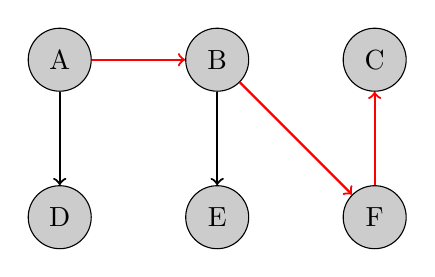
\begin{tikzpicture}[
            node/.style={circle, draw, fill=gray!40, minimum size=0.8cm},
            edge/.style={->, thick}
        ]
        % Create nodes
        \node[node] (A2) at (0,2) {A};
        \node[node] (B2) at (2,2) {B};
        \node[node] (C2) at (4,2) {C};
        \node[node] (D2) at (0,0) {D};
        \node[node] (E2) at (2,0) {E};
        \node[node] (F2) at (4,0) {F};
        
        % Create edges
        \draw[edge, red, thick] (A2) -- (B2);
        \draw[edge] (A2) -- (D2);
        \draw[edge] (B2) -- (E2);
        \draw[edge, red, thick] (B2) -- (F2);
        \draw[edge, red, thick] (F2) -- (C2);
        \end{tikzpicture}
        \caption{After BFS traversal, we can store the previous nodes in a hashmap $\{B \mapsto A, D \mapsto A, E \mapsto B, F \mapsto B, C \mapsto F\}$. From this we can see the path to get to $C$ is $A \mapsto B \mapsto F \mapsto C$ of length 3. }
        \label{fig:graph2}
      \end{subfigure}
      \caption{Comparison of two directed graphs with different path lengths from A to C.}
      \label{fig:graph-comparison}
    \end{figure}

    By construction, we can see that the path from A to C is always shorter for BFS than for DFS. 
  \end{definition}

\subsection{Trees} 

  Now we look at one special type of graph, called a \textit{tree}. 

  \begin{definition}[Trees]
    An undirected graph $G(V, E)$ is a \textbf{tree} iff $G$ is connected and has no cycles.\footnote{ Removing the first requirement gives us the definition of a \textbf{forest}, which is a collection of trees. }
    \begin{enumerate}
      \item The \textbf{root} of the tree is the top node. 
      \item The \textbf{leaf} of the tree are nodes that do not have children. 
      \item A \textbf{path} is any path from one node to another node. A simple path is a path that doesn't cross the same edge twice 
      \item The \textbf{height} of a node is the length of the longest downward path to a leaf from that node. 
      \item The \textbf{depth} of a node is the number of edges from the root to the node. 
      \item The \textbf{size} of the tree is the number of nodes $n$ it contains. 
    \end{enumerate}
  \end{definition}

  \begin{theorem}[Properties of Trees]
    If $G(V, E)$ is a tree, then 
    \begin{enumerate}
      \item There exists a $v \in V$ s.t. $d_v = 1$, called a \textbf{leaf node}. 
      \item $|E| = |V| - 1 = n - 1$. 
    \end{enumerate}
  \end{theorem}
  \begin{proof}
    The outlines are quite intuitive. 
    \begin{enumerate}
      \item There must be some leaf node since if there wasn't, then we would have a cycle. We can use proof by contradiction. 
      \item We can use proof by induction. We start off with one vertex and to construct a tree, we must add one edge and one vertex at every step, keeping this invariant.  
    \end{enumerate}
  \end{proof} 

  Now we can get to the elementary operations on a tree. 

  \begin{algo}[Insert Node to Tree] 
    Inserting is a bit ambiguous since we most also know \textit{where} to insert the value to. In general traversing this tree is $O(\log{n})$, and so we have the same runtime. 
    \begin{algorithmic}[1]
    \Procedure{Insert}{$root, key, value$}
      \If{$root = \text{null}$}
        \State \Return \text{new Node}$(key, value)$
      \EndIf
      \If{$key < root.key$}
        \State $root.left \gets \Call{Insert}{root.left, key, value}$
      \ElsIf{$key > root.key$}
        \State $root.right \gets \Call{Insert}{root.right, key, value}$
      \Else
        \State $root.value \gets value$ \Comment{Update if key already exists}
      \EndIf
      \State \Return $root$
    \EndProcedure
    \end{algorithmic}
  \end{algo}

  \begin{algo}[Remove Node in Tree]
    Removing is very similar, with also a runtime of $O(\log{n})$. 
    \begin{algorithmic}[1]
    \Procedure{Remove}{$root, key$}
      \If{$root = \text{null}$}
        \State \Return $\text{null}$
      \EndIf
      \If{$key < root.key$}
        \State $root.left \gets \Call{Remove}{root.left, key}$
      \ElsIf{$key > root.key$}
        \State $root.right \gets \Call{Remove}{root.right, key}$
      \Else \Comment{Node with the key found}
        \If{$root.left = \text{null}$}
          \State \Return $root.right$
        \ElsIf{$root.right = \text{null}$}
          \State \Return $root.left$
        \EndIf
        \State $root.key \gets \Call{FindMin}{root.right}$
        \State $root.right \gets \Call{Remove}{root.right, root.key}$
      \EndIf
      \State \Return $root$
    \EndProcedure
    \end{algorithmic}
  \end{algo}

  \begin{algo}[Modify Node in Tree]
    Same with modifying a node: $O(\log{n})$. 
    \begin{algorithmic}[1]
    \Procedure{Modify}{$root, key, newValue$}
      \If{$root = \text{null}$}
        \State \Return $\text{null}$ \Comment{Key not found}
      \EndIf
      \If{$key < root.key$}
        \State $root.left \gets \Call{Modify}{root.left, key, newValue}$
      \ElsIf{$key > root.key$}
        \State $root.right \gets \Call{Modify}{root.right, key, newValue}$
      \Else
        \State $root.value \gets newValue$ \Comment{Update value when key is found}
      \EndIf
      \State \Return $root$
    \EndProcedure
    \end{algorithmic}
  \end{algo}

  Since a node also has a specified depth and height, we should also know how to calculate this. 

  \begin{algo}[Height of Node]
    The height of a node is the longest downward path to a leaf from that node, so its height would be the maximum of the two heights of its children. A null node would have height $-1$, which is our base case. 
    \begin{algorithmic}[1]
    \Procedure{GetHeight}{$root$}
      \If{$root = \text{null}$}
        \State \Return $-1$
      \EndIf
      \State \Return $1 + \max(\Call{GetHeight}{root.\text{left}}, \Call{GetHeight}{root.\text{right}})$
    \EndProcedure
    \end{algorithmic}
  \end{algo}

  \begin{algo}[Depth of Node]
    The depth is quite hard to find recursively, but if we have a reference to the parent, then we can write 
    \begin{algorithmic}[1]
    \Procedure{Depth}{$node$}
      \If{$node = \text{null}$}
        \State \Return $-1$
      \Else
        \State \Return $1 + \Call{Depth}{node.\text{parent}}$
      \EndIf
    \EndProcedure
    \end{algorithmic}
  \end{algo}

\subsubsection{Binary Trees} 

  Most of the time, we work with \textit{binary trees}, which means that each node has has at most 2 children, denoted a \textit{left child} and \textit{right child}. 

  \begin{definition}[Binary Tree]
    A \textbf{binary tree} is a recursive data structure in which every node has up to two children, which we call the \textbf{left child} and \textbf{right child}. 

    \begin{figure}[H]
      \centering 
      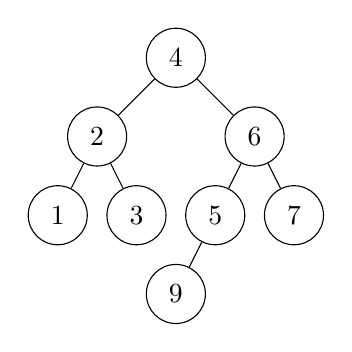
\begin{tikzpicture}[  every node/.style={    circle,    minimum size=0.75cm,    draw,    text centered,    anchor=center  }]
        \node (4) at (0,0) {4};
        \node (2) at (-1,-1) {2};
        \node (6) at (1,-1) {6};
        \node (1) at (-1.5,-2) {1};
        \node (3) at (-0.5,-2) {3};
        \node (5) at (0.5,-2) {5};
        \node (7) at (1.5,-2) {7};
        \node (9) at (0, -3) {9}; 
        \draw (4) -- (2);
        \draw (4) -- (6);
        \draw (2) -- (1);
        \draw (2) -- (3);
        \draw (6) -- (5);
        \draw (6) -- (7); 
        \draw (5) -- (9); 
      \end{tikzpicture}
      \caption{An example of a binary tree. The root is 4, with a max depth of 3. } 
      \label{fig:binary_tree}
    \end{figure}
  \end{definition} 

  A natural question is whether we can take this tree structure and retrieve all of its values. There are three recursive paradigms to do this, which differs by where the nonrecursive call is. 

  \begin{algo}[In Order Traversal]
    \textbf{In-Order traversal} tells us to print everything on the left of the node, then print the node, and then print everything on the right. 
    \begin{algorithmic}[1]
    \Procedure{InOrder}{$t$}
      \If{$t \neq \text{null}$}
        \State \Call{InOrder}{$t.\text{left}$}
        \State \textbf{print} $t.\text{info}$
        \State \Call{InOrder}{$t.\text{right}$}
      \EndIf
    \EndProcedure
    \end{algorithmic}
  \end{algo}

  \begin{algo}[PreOrder Traversal]
    \textbf{Pre-Order traversal} tells us to print the node itself first, then print all the ones on the left, and then print all the ones on the right. 
    \begin{algorithmic}[1]
    \Procedure{PreOrder}{$t$}
      \If{$t \neq \text{null}$}
        \State \textbf{print} $t.\text{info}$
        \State \Call{PreOrder}{$t.\text{left}$}
        \State \Call{PreOrder}{$t.\text{right}$}
      \EndIf
    \EndProcedure
    \end{algorithmic}
  \end{algo}

  \begin{algo}[PostOrder Traversal]
    \textbf{Post-Order traversal} tells us to print all the nodes on the left, then all ones on the right, and then the node itself. 
    \begin{algorithmic}[1]
    \Procedure{PostOrder}{$t$}
      \If{$t \neq \text{null}$}
        \State \Call{PostOrder}{$t.\text{left}$}
        \State \Call{PostOrder}{$t.\text{right}$}
        \State \textbf{print} $t.\text{info}$
      \EndIf
    \EndProcedure
    \end{algorithmic}
  \end{algo} 

  \begin{example}[Converting Tree to List]
    It's worth to go over an example here. Given the following binary tree, 

    \begin{figure}[H]
      \centering 
      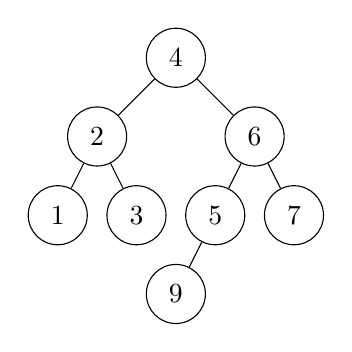
\begin{tikzpicture}[  every node/.style={    circle,    minimum size=0.75cm,    draw,    text centered,    anchor=center  }]
        \node (4) at (0,0) {4};
        \node (2) at (-1,-1) {2};
        \node (6) at (1,-1) {6};
        \node (1) at (-1.5,-2) {1};
        \node (3) at (-0.5,-2) {3};
        \node (5) at (0.5,-2) {5};
        \node (7) at (1.5,-2) {7};
        \node (9) at (0, -3) {9}; 
        \draw (4) -- (2);
        \draw (4) -- (6);
        \draw (2) -- (1);
        \draw (2) -- (3);
        \draw (6) -- (5);
        \draw (6) -- (7); 
        \draw (5) -- (9); 
      \end{tikzpicture}
      \caption{An example of a binary tree. The root is 4, with a max depth of 3. } 
      \label{fig:binary_tree_to_list}
    \end{figure}
    If we initialize a list and replace the print statement with an insert to the (end of the) list, then 
    \begin{enumerate}
      \item a in-order traversal produces: $[1, 2, 3, 4, 9, 5, 6, 7]$
      \item a pre-order traversal produces: $[4, 2, 1, 3, 6, 5, 9, 7]$
      \item a post-order traversal produces: $[1, 3, 2, 9, 5, 7, 6, 4]$
    \end{enumerate}
  \end{example}

  What we have described is a traversal method, and a natural question is to ask: Are these related to the more general DFS and BFS in any way? In fact it is. 

  \begin{theorem}[Tree Traversals and DFS]
    All forms of traversal are a specific variant of DFS starting from the root. 
    \begin{enumerate}
      \item A pre-order traversal prioritizes the left node to explore and is the common DFS variant used in general graph traversal.  
      \item An in-order traversal always prioritizes adding an unexplored left child to the stack, and if there is no left child, then the node is printed, and then the right child is pushed to the stack and explored. 
      \item A post-order traversal always prioritizes adding an unexplored left child to the stack, and if there is no left child, then the right child is pushed to the stack and explored. Once the right child is finished exploring the parent node is printed. 
    \end{enumerate}
  \end{theorem}

  So what does BFS do? There is another traversal which traverses the layers of each tree. 

  \begin{algo}[Level Order Traversal]
    \textbf{Level-order traversal} tells us to print all nodes of depth $0$, then all nodes of depth $1$, and so on.
    \begin{algorithmic}[1]
    \Procedure{LevelOrder}{$t$}
      \If{$t \neq \text{null}$}
        \State Create an empty queue $Q$
        \State Enqueue $t$ to $Q$
        \While{$Q$ is not empty}
          \State $node \gets$ Dequeue from $Q$
          \State \textbf{print} $node.\text{info}$
          \If{$node.\text{left} \neq \text{null}$}
            \State Enqueue $node.\text{left}$ to $Q$
          \EndIf
          \If{$node.\text{right} \neq \text{null}$}
            \State Enqueue $node.\text{right}$ to $Q$
          \EndIf
        \EndWhile
      \EndIf
    \EndProcedure
    \end{algorithmic}
  \end{algo}

\subsection{Heaps}

  A heap is sort of in between a sorted array and an unsorted array. 

  \begin{definition}[Binary Heap]
    A \textbf{binary heap} is a binary tree satisfying the following structural invariants: 
    \begin{enumerate}
      \item Maintain the \textbf{heap property} that every node is less than or equal to its successors, and 
      \item The \textbf{shape property} that the tree is complete (full except perhaps last level, in which case it should be filled from left to right. 
    \end{enumerate}

    \begin{figure}[H]
      \centering
      \begin{tikzpicture}[scale=0.7]
        \node[left] at (-2,0) {Depth 0};
        \node[left] at (-2,-2) {Depth 1};
        \node[left] at (-2,-4) {Depth 2};
        \node[left] at (-2,-6) {Depth 3};
        
        % Nodes
        % Depth 0
        \node[circle, draw, minimum size=0.8cm] (n1) at (5,0) {6};
        \node[below=0.2cm of n1, red] {1};
        
        % Depth 1
        \node[circle, draw, minimum size=0.8cm] (n2) at (2.5,-2) {10};
        \node[below=0.2cm of n2, red] {2};
        \node[circle, draw, minimum size=0.8cm] (n3) at (7.5,-2) {7};
        \node[below=0.2cm of n3, red] {3};
        
        % Depth 2
        \node[circle, draw, minimum size=0.8cm] (n4) at (1,-4) {17};
        \node[below=0.2cm of n4, red] {4};
        \node[circle, draw, minimum size=0.8cm] (n5) at (4,-4) {13};
        \node[below=0.2cm of n5, red] {5};
        \node[circle, draw, minimum size=0.8cm] (n6) at (6,-4) {9};
        \node[below=0.2cm of n6, red] {6};
        \node[circle, draw, minimum size=0.8cm] (n7) at (9,-4) {21};
        \node[below=0.2cm of n7, red] {7};
        
        % Depth 3
        \node[circle, draw, minimum size=0.8cm] (n8) at (0,-6) {19};
        \node[below=0.2cm of n8, red] {8};
        \node[circle, draw, minimum size=0.8cm] (n9) at (2,-6) {25};
        \node[below=0.2cm of n9, red] {9};
        
        % Edges
        \draw (n1) -- (n2);
        \draw (n1) -- (n3);
        \draw (n2) -- (n4);
        \draw (n2) -- (n5);
        \draw (n3) -- (n6);
        \draw (n3) -- (n7);
        \draw (n4) -- (n8);
        \draw (n4) -- (n9);
      \end{tikzpicture}
      \caption{Tree structure of a binary heap, with red labels representing the indices of the array structure mentioned below. }
      \label{fig:binary-heap}
    \end{figure}
  \end{definition}

  We should conceptually think of a binary heap as an underlying binary tree, but it is actually usually implemented with an array, and we can create a map from the heap to the array with the following indices. 

  \begin{figure}[H]
    \centering 
    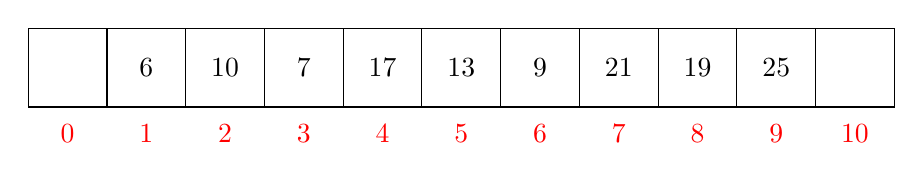
\begin{tikzpicture}
      \foreach \i in {0,...,10} {
        \draw (\i,0) rectangle +(1,1);
        \node[below] at (\i+0.5,-0.1) {\textcolor{red}{\i}};
      }
      
      % Add the values
      \node at (1.5,0.5) {6};
      \node at (2.5,0.5) {10};
      \node at (3.5,0.5) {7};
      \node at (4.5,0.5) {17};
      \node at (5.5,0.5) {13};
      \node at (6.5,0.5) {9};
      \node at (7.5,0.5) {21};
      \node at (8.5,0.5) {19};
      \node at (9.5,0.5) {25};
    \end{tikzpicture}
    \caption{When 1-indexing, for node with index $k$, the left child is index $2k$, the right child is index $2k + 1$, and the parent is index $k/2$ (where this is integer division). } 
    \label{fig:binary_heap_array}
  \end{figure}

  Implementing peek is easy, since we just return the first index, but it can be quite tricky to maintain this invariant after an arbitrary sequence of add/remove operations. 
  \begin{enumerate}
    \item To add values to a heap, we add to the first open position in the last level of the tree (to maintain the shape property), and then swap with the parent is the heap property is violated. If we are swapping with the parent at most $\log(N)$ times, then the add property has $O(\log(N))$ complexity. 

    \begin{figure}[H]
      \centering
      \begin{subfigure}[b]{0.48\textwidth}
      \centering
        \begin{tikzpicture}[scale=0.7]
          % Nodes
          % Depth 0
          \node[circle, draw, minimum size=0.8cm] (n1) at (5,0) {6};
          \node[below=0.2cm of n1, red] {1};
          
          % Depth 1
          \node[circle, draw, minimum size=0.8cm] (n2) at (2.5,-2) {10};
          \node[below=0.2cm of n2, red] {2};
          \node[circle, draw, minimum size=0.8cm] (n3) at (7.5,-2) {7};
          \node[below=0.2cm of n3, red] {3};
          
          % Depth 2
          \node[circle, draw, minimum size=0.8cm] (n4) at (1,-4) {17};
          \node[below=0.2cm of n4, red] {4};
          \node[circle, draw, minimum size=0.8cm] (n5) at (4,-4) {13};
          \node[below=0.2cm of n5, red] {5};
          \node[circle, draw, minimum size=0.8cm] (n6) at (6,-4) {9};
          \node[below=0.2cm of n6, red] {6};
          \node[circle, draw, minimum size=0.8cm] (n7) at (9,-4) {21};
          \node[below=0.2cm of n7, red] {7};
          
          % Depth 3
          \node[circle, draw, minimum size=0.8cm] (n8) at (0,-6) {19};
          \node[below=0.2cm of n8, red] {8};
          \node[circle, draw, minimum size=0.8cm] (n9) at (2,-6) {25};
          \node[below=0.2cm of n9, red] {9};
          \node[circle, draw, minimum size=0.8cm, fill=yellow] (n10) at (3.5,-6) {11};
          \node[below=0.2cm of n10, red] {10};
          
          % Edges
          \draw (n1) -- (n2);
          \draw (n1) -- (n3);
          \draw (n2) -- (n4);
          \draw (n2) -- (n5);
          \draw (n3) -- (n6);
          \draw (n3) -- (n7);
          \draw (n4) -- (n8);
          \draw (n4) -- (n9);
          \draw (n5) -- (n10);
        \end{tikzpicture}
        \caption{Add the 11 node to the tree by inserting in the lowest depth, from left to right.}
        \label{fig:first_add}
      \end{subfigure}
      \hfill 
      \begin{subfigure}[b]{0.48\textwidth}
      \centering
        \begin{tikzpicture}[scale=0.7]
          % Nodes
          % Depth 0
          \node[circle, draw, minimum size=0.8cm] (n1) at (5,0) {6};
          \node[below=0.2cm of n1, red] {1};
          
          % Depth 1
          \node[circle, draw, minimum size=0.8cm] (n2) at (2.5,-2) {10};
          \node[below=0.2cm of n2, red] {2};
          \node[circle, draw, minimum size=0.8cm] (n3) at (7.5,-2) {7};
          \node[below=0.2cm of n3, red] {3};
          
          % Depth 2
          \node[circle, draw, minimum size=0.8cm] (n4) at (1,-4) {17};
          \node[below=0.2cm of n4, red] {4};
          \node[circle, draw, minimum size=0.8cm, fill=yellow] (n5) at (4,-4) {11};
          \node[below=0.2cm of n5, red] {5};
          \node[circle, draw, minimum size=0.8cm] (n6) at (6,-4) {9};
          \node[below=0.2cm of n6, red] {6};
          \node[circle, draw, minimum size=0.8cm] (n7) at (9,-4) {21};
          \node[below=0.2cm of n7, red] {7};
          
          % Depth 3
          \node[circle, draw, minimum size=0.8cm] (n8) at (0,-6) {19};
          \node[below=0.2cm of n8, red] {8};
          \node[circle, draw, minimum size=0.8cm] (n9) at (2,-6) {25};
          \node[below=0.2cm of n9, red] {9};
          \node[circle, draw, minimum size=0.8cm] (n10) at (3.5,-6) {13};
          \node[below=0.2cm of n10, red] {10};
          
          % Edges
          \draw (n1) -- (n2);
          \draw (n1) -- (n3);
          \draw (n2) -- (n4);
          \draw (n2) -- (n5);
          \draw (n3) -- (n6);
          \draw (n3) -- (n7);
          \draw (n4) -- (n8);
          \draw (n4) -- (n9);
          \draw (n5) -- (n10);
        \end{tikzpicture}
        \caption{Keep swapping the added node with its ancestor if the node is smaller.}
        \label{fig:then_swap}
      \end{subfigure}
      \caption{Visual of how to add nodes to a heap. }
      \label{fig:head_add}
    \end{figure} 

    \item We remove the first (minimal) value, we first replace the root with the last node in the heap, and while the heap property is violated, we swap with the smaller child. There are two choices, the left or right child, in which we can swap. But we must always swap with the \textbf{smaller child}, since we swapped with the bigger child, then this bigger child would be larger than the smaller one, violating the heap property. Since a complete binary tree always has height $O(\log(N))$, remove also "traverses" one root-leaf path, and so its runtime complexity is $O(\log(N))$, too. hi

    \begin{figure}[H]
      \centering
      \begin{subfigure}[b]{0.48\textwidth}
      \centering
        \begin{tikzpicture}[scale=0.7]
          % Nodes
          % Depth 0
          \node[circle, draw, minimum size=0.8cm] (n1) at (5,0) {25};
          \node[below=0.2cm of n1, red] {1};
          
          % Depth 1
          \node[circle, draw, minimum size=0.8cm] (n2) at (2.5,-2) {10};
          \node[below=0.2cm of n2, red] {2};
          \node[circle, draw, minimum size=0.8cm] (n3) at (7.5,-2) {7};
          \node[below=0.2cm of n3, red] {3};
          
          % Depth 2
          \node[circle, draw, minimum size=0.8cm] (n4) at (1,-4) {17};
          \node[below=0.2cm of n4, red] {4};
          \node[circle, draw, minimum size=0.8cm] (n5) at (4,-4) {13};
          \node[below=0.2cm of n5, red] {5};
          \node[circle, draw, minimum size=0.8cm] (n6) at (6,-4) {9};
          \node[below=0.2cm of n6, red] {6};
          \node[circle, draw, minimum size=0.8cm] (n7) at (9,-4) {21};
          \node[below=0.2cm of n7, red] {7};
          
          % Depth 3
          \node[circle, draw, minimum size=0.8cm] (n8) at (0,-6) {19};
          \node[below=0.2cm of n8, red] {8};
          
          % Edges
          \draw (n1) -- (n2);
          \draw (n1) -- (n3);
          \draw (n2) -- (n4);
          \draw (n2) -- (n5);
          \draw (n3) -- (n6);
          \draw (n3) -- (n7);
          \draw (n4) -- (n8);
        \end{tikzpicture}
        \caption{Pop 6 node and replace it with last node 25.}
        \label{fig:remove-heap-step1}
      \end{subfigure}
      \hfill 
      \begin{subfigure}[b]{0.48\textwidth}
      \centering
        \begin{tikzpicture}[scale=0.7]
          % Nodes
          % Depth 0
          \node[circle, draw, minimum size=0.8cm] (n1) at (5,0) {7};
          \node[below=0.2cm of n1, red] {1};
          
          % Depth 1
          \node[circle, draw, minimum size=0.8cm] (n2) at (2.5,-2) {10};
          \node[below=0.2cm of n2, red] {2};
          \node[circle, draw, minimum size=0.8cm] (n3) at (7.5,-2) {25};
          \node[below=0.2cm of n3, red] {3};
          
          % Depth 2
          \node[circle, draw, minimum size=0.8cm] (n4) at (1,-4) {17};
          \node[below=0.2cm of n4, red] {4};
          \node[circle, draw, minimum size=0.8cm] (n5) at (4,-4) {13};
          \node[below=0.2cm of n5, red] {5};
          \node[circle, draw, minimum size=0.8cm] (n6) at (6,-4) {9};
          \node[below=0.2cm of n6, red] {6};
          \node[circle, draw, minimum size=0.8cm] (n7) at (9,-4) {21};
          \node[below=0.2cm of n7, red] {7};
          
          % Depth 3
          \node[circle, draw, minimum size=0.8cm] (n8) at (0,-6) {19};
          \node[below=0.2cm of n8, red] {8};
          
          % Edges
          \draw (n1) -- (n2);
          \draw (n1) -- (n3);
          \draw (n2) -- (n4);
          \draw (n2) -- (n5);
          \draw (n3) -- (n6);
          \draw (n3) -- (n7);
          \draw (n4) -- (n8);
        \end{tikzpicture}
        \caption{Swap the 25 node with the smaller 7 node.}
        \label{fig:remove-heap-step2}
      \end{subfigure}

      \begin{subfigure}[b]{0.48\textwidth}
      \centering
        \begin{tikzpicture}[scale=0.7]
          % Nodes
          % Depth 0
          \node[circle, draw, minimum size=0.8cm] (n1) at (5,0) {7};
          \node[below=0.2cm of n1, red] {1};
          
          % Depth 1
          \node[circle, draw, minimum size=0.8cm] (n2) at (2.5,-2) {10};
          \node[below=0.2cm of n2, red] {2};
          \node[circle, draw, minimum size=0.8cm] (n3) at (7.5,-2) {9};
          \node[below=0.2cm of n3, red] {3};
          
          % Depth 2
          \node[circle, draw, minimum size=0.8cm] (n4) at (1,-4) {17};
          \node[below=0.2cm of n4, red] {4};
          \node[circle, draw, minimum size=0.8cm] (n5) at (4,-4) {13};
          \node[below=0.2cm of n5, red] {5};
          \node[circle, draw, minimum size=0.8cm] (n6) at (6,-4) {25};
          \node[below=0.2cm of n6, red] {6};
          \node[circle, draw, minimum size=0.8cm] (n7) at (9,-4) {21};
          \node[below=0.2cm of n7, red] {7};
          
          % Depth 3
          \node[circle, draw, minimum size=0.8cm] (n8) at (0,-6) {19};
          \node[below=0.2cm of n8, red] {8};
          
          % Edges
          \draw (n1) -- (n2);
          \draw (n1) -- (n3);
          \draw (n2) -- (n4);
          \draw (n2) -- (n5);
          \draw (n3) -- (n6);
          \draw (n3) -- (n7);
          \draw (n4) -- (n8);
        \end{tikzpicture}
        \caption{Swap the 25 node with the smaller 9 node.}
        \label{fig:remove-heap-step3}
      \end{subfigure}

      \caption{Binary heap restructuring during deletion operation}
      \label{fig:remove-heap}
    \end{figure}
    
    \item The decreaseKey operation just takes an arbitrary node and decreases its value to some other integer. In this case, it wouldn't violate the shape property, and to restore the heap property, we just put swap it with its parent if the new value is smaller than its parent, making this operation $O(\log(N))$. 
  \end{enumerate}

  \begin{definition}[Priority Queues]
    A priority queue simply adds things according to their priority. Every time we add an element, it looks at where the element should go to keep the list sorted. If we want to dequeue, then we just remove the first element of the list. If we implement a priority queue with a heap, we have
    \begin{enumerate}
      \item Adding a new value is $O(\log N)$. 
      \item Removing a specific value is $O(\log N)$. 
      \item Peek returns the minimal element and is $O(1)$. 
      \item Checking if a value is contained in a priority queue is ?. 
    \end{enumerate}
  \end{definition}

\subsection{Binary Search Trees}

  \begin{definition}[Binary Search Tree]
    A binary tree is a \textbf{binary search tree} if for every node, the left subtree values are all less than the node's value, and the right subtree values are all greater than the node's value. That is, the nodes are in order, and if we called $\texttt{inOrder(root)}$ on the tree, then we would get a sorted list, which allows for efficient search. 
  \end{definition}

  Adding elements to a binary search tree is also very similar. But note that the order in which we add elements to the binary search tree will matter, since it can either make the tree \textbf{balanced} or \textbf{unbalanced}. 

  \begin{figure}[H]
    \centering 
    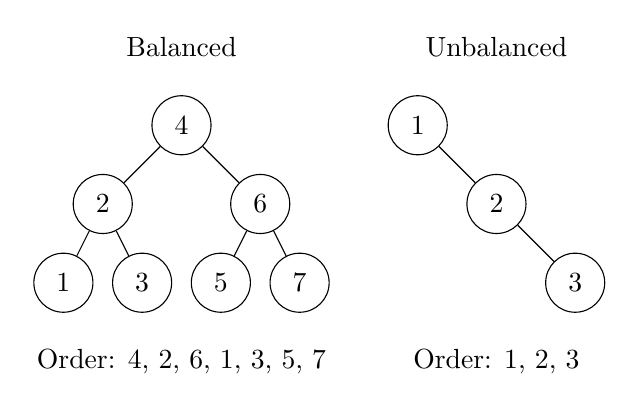
\begin{tikzpicture}[ integer/.style={    draw,    circle,    minimum size=0.75cm,    inner sep=0pt,    text centered,    anchor=center  }]
      % Balanced tree
      \node[integer] (4) at (0,0) {4};
      \node[integer] (2) at (-1,-1) {2};
      \node[integer] (6) at (1,-1) {6};
      \node[integer] (1) at (-1.5,-2) {1};
      \node[integer] (3) at (-0.5,-2) {3};
      \node[integer] (5) at (0.5,-2) {5};
      \node[integer] (7) at (1.5,-2) {7};
      \draw (4) -- (2);
      \draw (4) -- (6);
      \draw (2) -- (1);
      \draw (2) -- (3);
      \draw (6) -- (5);
      \draw (6) -- (7);

      % Caption for balanced tree
      \node at (0,1) {Balanced};
      \node at (0,-3) {Order: 4, 2, 6, 1, 3, 5, 7};

      % Unbalanced tree
      \node[integer] (1') at (3,0) {1};
      \node[integer] (2') at (4,-1) {2};
      \node[integer] (3') at (5,-2) {3};
      \draw (1') -- (2');
      \draw (2') -- (3');

      % Caption for unbalanced tree
      \node at (4,1) {Unbalanced};
      \node at (4,-3) {Order: 1, 2, 3};
    \end{tikzpicture}
    \caption{Comparison of balanced and unbalanced binary trees. In a balanced case, contains/add will be $O(\log(N))$, while in an unbalanced case, we will have $O(N)$.}
    \label{fig:trees}
  \end{figure}

  \begin{definition}[Binary Search]
    Given that we have a sorted list (this is important!), we can search for the index of an element in $O(\log{n})$ time. We want the loop invariant "if the target is in the array/list, it is in the range [low, high]." Let us have a list of $N$ elements, and at every step, we either 
    \begin{enumerate}
      \item get our desired element and its index, or 
      \item cut down our search space by half
    \end{enumerate}
  \end{definition}

  Now, we have learned how we can implement a priority queue using a binary heap. This is also possible to use a binary search tree, since it's easy to get the minimal element for adding and removing, but there are three things that make it difficult: 
  \begin{enumerate}
      \item all elements must be unique 
      \item it is not array-based, and so uses more memory and higher constant factors on runtime 
      \item it is much harder to implement with guarantees that the tree will be balanced. This makes it difficult since if we want to search through a balanced BST, it is $O(\log(N))$, but if it turns out to be unbalanced, then it is $O(N)$. 
  \end{enumerate}
  Therefore, while a balanced tree may be efficient on average, in the worst case the linear complexity is not tolerable. Therefore, we must implement a binary search tree that will do extra work to ensure that they are approximately balanced. This is where \textit{red-black trees}, which are a special type of binary search trees, come in.  

  \begin{definition}[Red-Black Tree]
    \textbf{Red-Black Trees} are binary search trees consisting of nodes that are labeled either red or black that satisfy the following properties: 
    \begin{enumerate}
      \item The root is black 
      \item A red node cannot have red children 
      \item From any node, all paths to null descendants must have the same number of black nodes. (Null is considered to be a black node)
    \end{enumerate}

    \begin{figure}[H]
      \centering
      \begin{subfigure}[b]{0.32\textwidth}
      \centering
        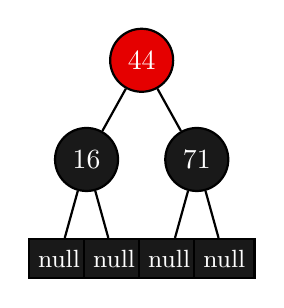
\begin{tikzpicture}[
          scale=0.7,
          red_node/.style={circle, draw, thick, fill=red!90!black, text=white, minimum size=0.8cm},
          black_node/.style={circle, draw, thick, fill=black!90, text=white, minimum size=0.8cm},
          null_node/.style={rectangle, draw, thick, fill=black!90, text=white, minimum size=0.5cm, font=\small},
          edge/.style={draw, thick, -}
        ]
        % First tree (invalid red-black tree)
        % Nodes
        \node[red_node] (n44) at (0,0) {44};
        \node[black_node] (n16) at (-1,-1.8) {16};
        \node[black_node] (n71) at (1,-1.8) {71};
        \node[null_node] (n16l) at (-1.5,-3.6) {null};
        \node[null_node] (n16r) at (-0.5,-3.6) {null};
        \node[null_node] (n71l) at (0.5,-3.6) {null};
        \node[null_node] (n71r) at (1.5,-3.6) {null};
        
        % Edges
        \draw[edge] (n44) -- (n16);
        \draw[edge] (n44) -- (n71);
        \draw[edge] (n16) -- (n16l);
        \draw[edge] (n16) -- (n16r);
        \draw[edge] (n71) -- (n71l);
        \draw[edge] (n71) -- (n71r);
        \end{tikzpicture}
        \caption{Invalid: Root node is red, violating the property that the root must be black.}
        \label{fig:rb-invalid1}
      \end{subfigure}
      \hfill 
      \begin{subfigure}[b]{0.32\textwidth}
      \centering
        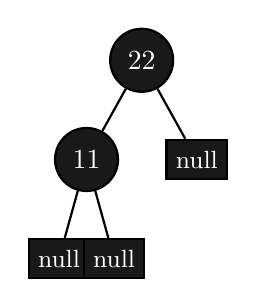
\begin{tikzpicture}[
          scale=0.7,
          red_node/.style={circle, draw, thick, fill=red!90!black, text=white, minimum size=0.8cm},
          black_node/.style={circle, draw, thick, fill=black!90, text=white, minimum size=0.8cm},
          null_node/.style={rectangle, draw, thick, fill=black!90, text=white, minimum size=0.5cm, font=\small},
          edge/.style={draw, thick, -}
        ]
        % Second tree (invalid red-black tree)
        % Nodes
        \node[black_node] (n22) at (0,0) {22};
        \node[black_node] (n11) at (-1,-1.8) {11};
        \node[null_node] (n22r) at (1,-1.8) {null};
        \node[null_node] (n11l) at (-1.5,-3.6) {null};
        \node[null_node] (n11r) at (-0.5,-3.6) {null};
        
        % Edges
        \draw[edge] (n22) -- (n11);
        \draw[edge] (n22) -- (n22r);
        \draw[edge] (n11) -- (n11l);
        \draw[edge] (n11) -- (n11r);
        \end{tikzpicture}
        \caption{Invalid: Path (22,null) has 2 black nodes, but path (22,11,null) has 3, violating the black-depth property.}
        \label{fig:rb-invalid2}
      \end{subfigure}
      \hfill 
      \begin{subfigure}[b]{0.32\textwidth}
      \centering
        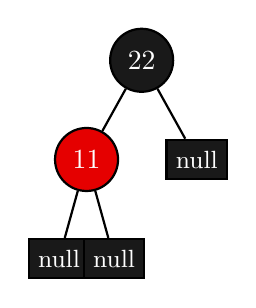
\begin{tikzpicture}[
          scale=0.7,
          red_node/.style={circle, draw, thick, fill=red!90!black, text=white, minimum size=0.8cm},
          black_node/.style={circle, draw, thick, fill=black!90, text=white, minimum size=0.8cm},
          null_node/.style={rectangle, draw, thick, fill=black!90, text=white, minimum size=0.5cm, font=\small},
          edge/.style={draw, thick, -}
        ]
        % Third tree (valid red-black tree)
        % Nodes
        \node[black_node] (n22) at (0,0) {22};
        \node[red_node] (n11) at (-1,-1.8) {11};
        \node[null_node] (n22r) at (1,-1.8) {null};
        \node[null_node] (n11l) at (-1.5,-3.6) {null};
        \node[null_node] (n11r) at (-0.5,-3.6) {null};
        
        % Edges
        \draw[edge] (n22) -- (n11);
        \draw[edge] (n22) -- (n22r);
        \draw[edge] (n11) -- (n11l);
        \draw[edge] (n11) -- (n11r);
        \end{tikzpicture}
        \caption{Valid: Root is black, reds have no red children, all paths from node to null have same black counts.}
        \label{fig:rb-valid}
      \end{subfigure}
      \caption{Examples and non-examples of red-black trees.}
      \label{fig:red-black-tree-examples}
    \end{figure}

    Remember that red black trees are also just binary search trees, and so some of the operations are the same.  
    \begin{enumerate}
      \item contains (search) method is the exact same thing as BST 
      \item The add method needs to be slightly modified, since after we add, we need to make sure that the resulting tree is a red-black tree. This is done in three steps: 
      \begin{enumerate}
        \item Run the regular BST add 
        \item Color the new node red 
        \item Fix the tree to reestablish red-black tree properties. This is extremely complicated with different cases, but it all essentially uses some sort of recoloring and a (right or left) rotation of the tree. 
      \end{enumerate}
    \end{enumerate}
  \end{definition}

  Note that there are binary search trees that cannot be turned into a red-black tree. 

  \begin{figure}[H]
    \centering
    \begin{subfigure}[b]{0.24\textwidth}
    \centering
      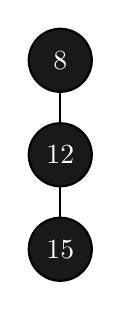
\begin{tikzpicture}[
        scale=0.6,
        red_node/.style={circle, draw, thick, fill=red!90!black, text=white, minimum size=0.8cm},
        black_node/.style={circle, draw, thick, fill=black!90, text=white, minimum size=0.8cm},
        edge/.style={draw, thick, -}
      ]
      % First tree - all black
      % Nodes
      \node[black_node] (n8) at (0,0) {8};
      \node[black_node] (n12) at (0,-2) {12};
      \node[black_node] (n15) at (0,-4) {15};
      
      % Edges
      \draw[edge] (n8) -- (n12);
      \draw[edge] (n12) -- (n15);
      \end{tikzpicture}
      \caption{Too many black nodes on right compared to left paths}
      \label{fig:rb-violation1}
    \end{subfigure}
    \hfill 
    \begin{subfigure}[b]{0.24\textwidth}
    \centering
      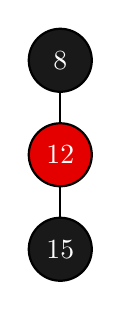
\begin{tikzpicture}[
        scale=0.6,
        red_node/.style={circle, draw, thick, fill=red!90!black, text=white, minimum size=0.8cm},
        black_node/.style={circle, draw, thick, fill=black!90, text=white, minimum size=0.8cm},
        edge/.style={draw, thick, -}
      ]
      % Second tree - middle red
      % Nodes
      \node[black_node] (n8) at (0,0) {8};
      \node[red_node] (n12) at (0,-2) {12};
      \node[black_node] (n15) at (0,-4) {15};
      
      % Edges
      \draw[edge] (n8) -- (n12);
      \draw[edge] (n12) -- (n15);
      \end{tikzpicture}
      \caption{Too many black nodes on right compared to left paths}
      \label{fig:rb-violation2}
    \end{subfigure}
    \hfill 
    \begin{subfigure}[b]{0.24\textwidth}
    \centering
      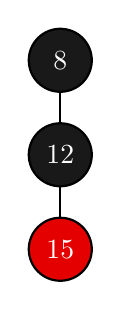
\begin{tikzpicture}[
        scale=0.6,
        red_node/.style={circle, draw, thick, fill=red!90!black, text=white, minimum size=0.8cm},
        black_node/.style={circle, draw, thick, fill=black!90, text=white, minimum size=0.8cm},
        edge/.style={draw, thick, -}
      ]
      % Third tree - bottom red
      % Nodes
      \node[black_node] (n8) at (0,0) {8};
      \node[black_node] (n12) at (0,-2) {12};
      \node[red_node] (n15) at (0,-4) {15};
      
      % Edges
      \draw[edge] (n8) -- (n12);
      \draw[edge] (n12) -- (n15);
      \end{tikzpicture}
      \caption{Too many black nodes on right compared to left paths}
      \label{fig:rb-violation3}
    \end{subfigure}
    \hfill 
    \begin{subfigure}[b]{0.24\textwidth}
    \centering
      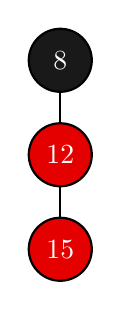
\begin{tikzpicture}[
        scale=0.6,
        red_node/.style={circle, draw, thick, fill=red!90!black, text=white, minimum size=0.8cm},
        black_node/.style={circle, draw, thick, fill=black!90, text=white, minimum size=0.8cm},
        edge/.style={draw, thick, -}
      ]
      % Fourth tree - middle and bottom red
      % Nodes
      \node[black_node] (n8) at (0,0) {8};
      \node[red_node] (n12) at (0,-2) {12};
      \node[red_node] (n15) at (0,-4) {15};
      
      % Edges
      \draw[edge] (n8) -- (n12);
      \draw[edge] (n12) -- (n15);
      \end{tikzpicture}
      \caption{Red node with red child not allowed}
      \label{fig:rb-violation4}
    \end{subfigure}
    \caption{Examples of Red-Black Tree violations.}
    \label{fig:red-black-tree-violations}
  \end{figure}

  This is intentional because red-black tree properties guarantee approximate balance. If we can turn a binary search tree into a red-black tree, then it logically follows that the original BST was approximately balanced. Note that a red black tree does not make searching asymptotically faster in any way; it just takes care of the worst-case. 

\subsection{Tries}

